\section{Timing Performances}
\label{sec:timing}

We now study the timing performances and coincidences of the two detectors. To do so, we first compute the difference between the recorded timing of each event of a channel with the timing of all the events from the other, and then take into account only the pair of events with the smallest time difference. Lastly, we plot this difference in a histogram in order to obtain the spectra of the time differences between events read from the two detectors. \\
For this analysis we use $^{22}$Na, as the two gammas produced in the decay are emitted simultaneously in opposite direction: thus, if a detector sees one gamma, we expect the other to detect one as well. \\

The spectrum in fig.\ref{fig:timing} shows that we have a constant distribution of time differences, which represents the non-correlated events background, with a peak around the zero representing the events in coincidence. Since the time difference for event in coincidence should be zero, we can consider the width of the peak as the timing resolution of the detectors. \\
The histogram is fit with eq.\ref{eq:fit_time}, where C is the position of the highest bin, since the peak clearly decays exponentially. 

\begin{equation}\label{eq:fit_time}
    f(x)= 
\begin{cases}
    a+b \cdot e^{\frac{(x-C)+d}{e}}& \text{if } x<C\\
    a+b \cdot e^{\frac{-(x-C)+d}{e}}              & \text{if } x \geq C
\end{cases}
\end{equation} 

\begin{figure}[H]
    \centering
    \includegraphics[scale=0.5]{Images/analysis/timing/time_response.pdf}
    \caption{Spectra of the time response of the detector for the source of $^{22}$Na. The best fit is shown as the red line, while the unrelated events region is shaded in red.}
    \label{fig:timing}
\end{figure}
 
Since the  peak is not gaussian, we decide to consider the width of the distribution as the difference between the two points where the derivative of the fit is equal to $e^{-6}$, $t_{0}^{\pm}$, shown in tab. \ref{table:t0}. The choice of $e^{-6}$ holds no particular physical meaning, but has been decided arbitrarily to have a reference value close enough to zero that provided reasonable results. In fig.\ref{fig:timing} the rejected region, corresponding to unrelated events, is highlighted along with the fitting function.

\begin{table}[ht]
    \centering
    \begin{tabular}{|c|c|c|c|c|}
    \hline
     & \multicolumn{2}{|c|}{Channel 0} & \multicolumn{2}{|c|}{Channel 1}\\
    \hline
    Source distance& $t_{0}^{-}$ [ns] & $t_{0}^{+}$ [ns] & $t_{0}^{-}$ [ns] & $t_{0}^{+}$ [ns] \\
    \hline
    10 cm& -13.7 & 19.7 & -17.7 & 15.7 \\
    15 cm& -13.1 & 19.1 & -17.1 & 15.1 \\
    20 cm& -13.3 & 19.3 & -17.3 & 15.3 \\
    Mean&  -13.4& 19.4& -17.4 & 15.4 \\
    \hline
    \end{tabular}
    \caption{Values that contain the coincidence region in the timing spectra, for detector 0 and 1, at different distances of the source. The last row shows the average between the different distances.}
    \label{table:t0}
\end{table}

Taking the average value of $t_{0}^{\pm}$, for both channels, we can estimate the width of the region, resulting in $ \Delta t_{ch0}=16.4$ ns and $\Delta t_{ch1}=16.4$ ns. We will thus considere a pair of events from channel 0 and 1 in coincidence if the time difference between them was less than 16 ns. \\
Note that the interval is the same for both detector, meaning they have the same time resolution as expected, but the ranges of coincindence shift from one channel to the other. This may be due to the fact that the source could have been placed not exactly in the center.

The effect of imposing the timing coincidence is shown in figure \ref{fig:T_effect_Na} and \ref{fig:T_effect_Co}, where in the subfigures \ref{fig:Na_ee} and \ref{fig:Co_ee} we can see the corresponding energies between the events in the two channel that have the smallest timing difference. We can observe, that without imposing the timing coincidence condition, we see correlation between peaks happening simoultaneously, but also with other energy values that are not necessarily in coincidence, as the one of the intrinsic radioactivity of the detector, around 1400 keV, or the one at 1275 keV for $^{22}$Na.
When we impose the timing coincidences, fig. \ref{fig:Na_ee_coinc} and \ref{fig:Co_ee_coinc}, we see that the only correlation left is only the one corresponding to events happening simultaneously, the two peaks at 511 keV for $^{22}$Na and the peaks at 1332 keV and 1173 keV for $^{60}$Co. So when one detector sees a peak the other sees the other peak.
\begin{figure}[H]
	\begin{minipage}[c]{0.5\linewidth}
	\subfloat[][No timing coincidence.]{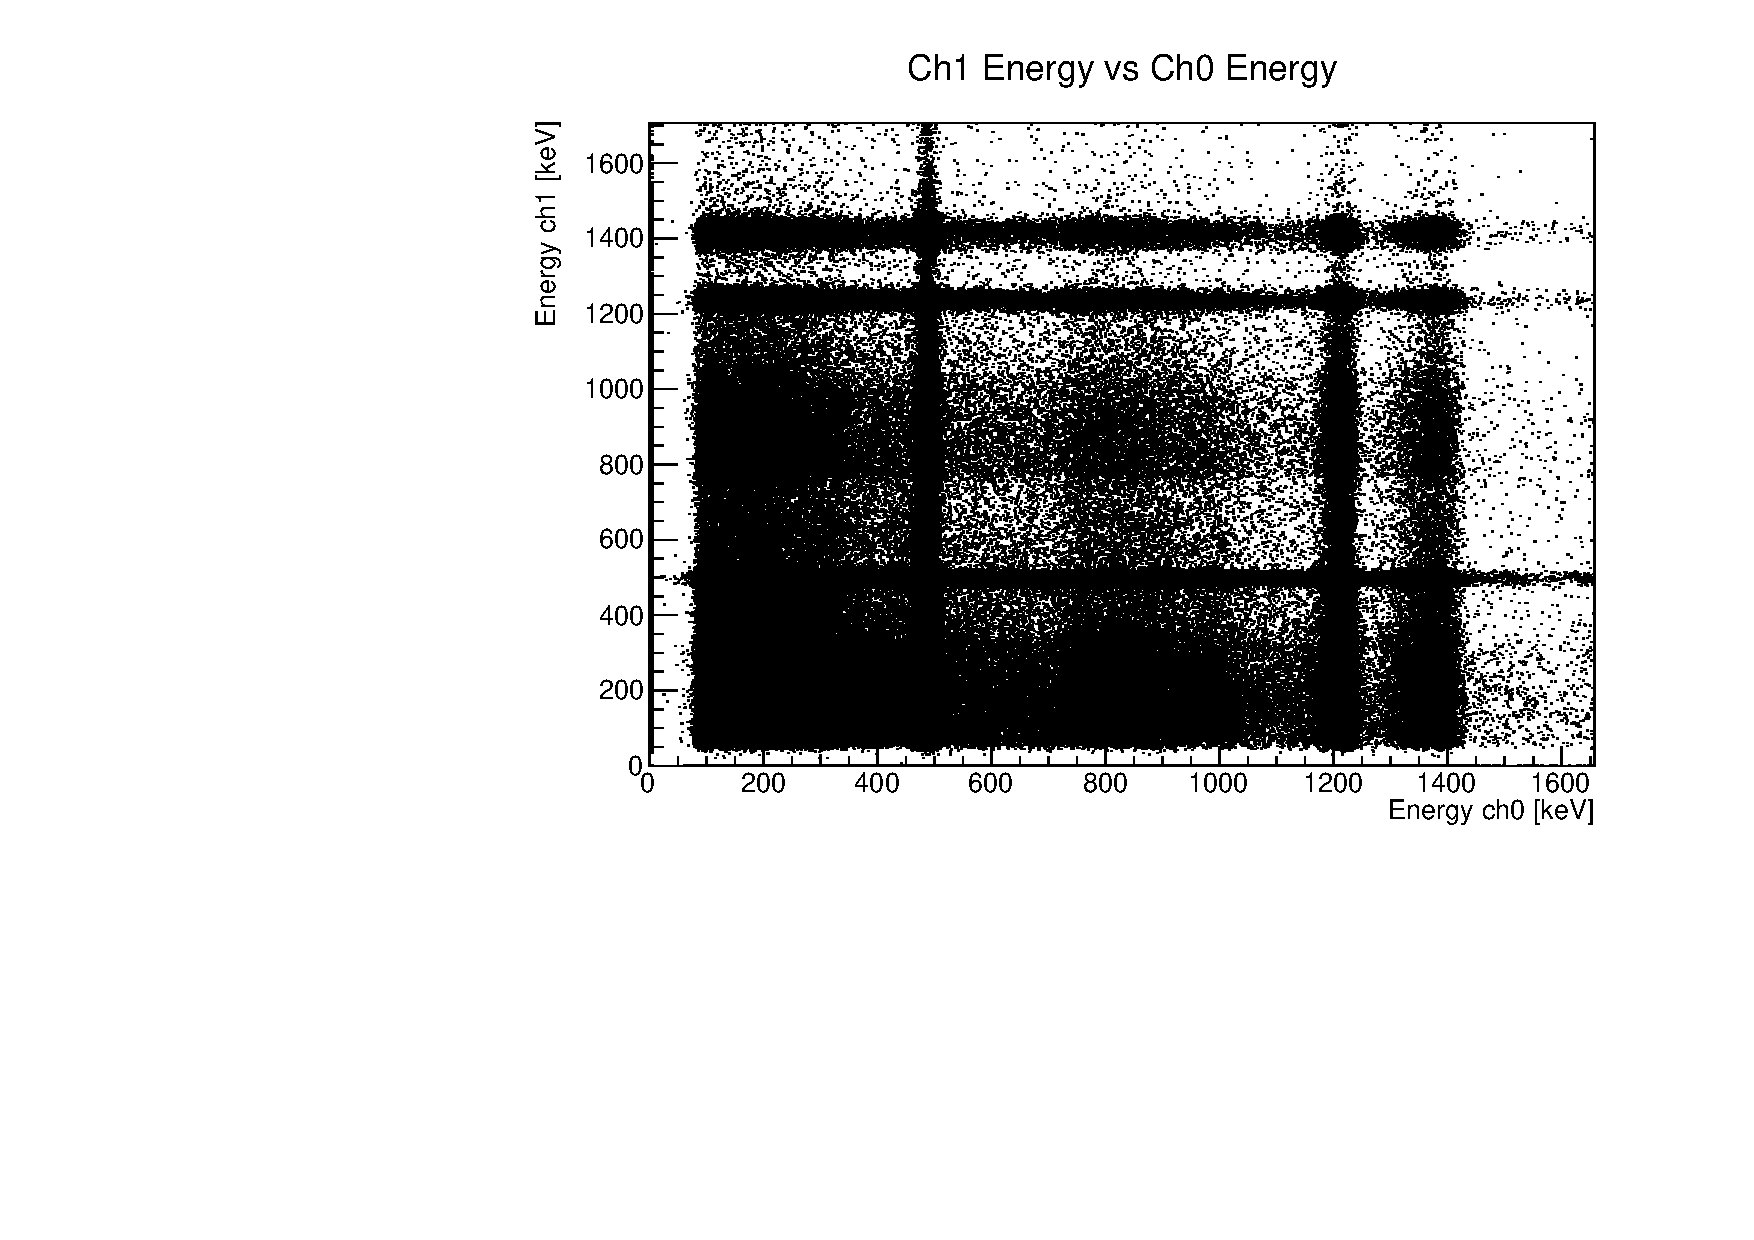
\includegraphics[width=0.9\textwidth]{Images/analysis/timing/Na_e1_vs_e2.pdf} \label{fig:Na_ee} }
	\end{minipage}
	\begin{minipage}[]{0.5\linewidth}
	\centering
	\subfloat[][Timing coincidence.]{\includegraphics[width=0.9\textwidth]{Images/analysis/timing/Na_e1_vs_e2_coinc.pdf}  \label{fig:Na_ee_coinc} }
	\end{minipage}
	\caption{Histograms showing the correlation between the energy spectra of channel 0 and channel 1, without and with the imposition of timing coincidence, for the $^{22}$Na source}
    \label{fig:T_effect_Na}
	\end{figure}
 \begin{figure}[H]
	\begin{minipage}[c]{0.5\linewidth}
	\subfloat[][No timing coincidence.]{\includegraphics[width=0.9\textwidth]{Images/analysis/timing/Co_e1_vs_e2.pdf} \label{fig:Co_ee} }
	\end{minipage}
	\begin{minipage}[]{0.5\linewidth}
	\centering
	\subfloat[][Timing coincidence.]{\includegraphics[width=0.9\textwidth]{Images/analysis/timing/Co_e1_vs_e2_coinc.pdf}  \label{fig:Co_ee_coinc} }
	\end{minipage}
	\caption{Histograms showing the correlation between the energy spectra of channel 0 and channel 1, without and with the imposition of timing coincidence, for the $^{60}$Co source}
    \label{fig:T_effect_Co}
	\end{figure}



\label{sec:timing}